\documentclass[9pt,xcolor=table]{beamer}
\usepackage[latin1]{inputenc}
\usepackage[english]{babel}
% \usepackage{graphics}
\usepackage{graphicx}
\usepackage{hyperref}
\usepackage{units}
\usepackage{amsmath}
\usepackage{amsfonts}
\usepackage{amssymb}
\usepackage{color, colortbl}
\usepackage{amsmath}
%\usepackage{wrapfig}
\usepackage[normalem]{ulem}
%\usepackage{multirow}
\usepackage{verbments}
\usepackage{textcomp}

\usetheme{MPICBG}

\def\cpp{\texttt{C++}}
\def\cpu{\texttt{CPU}}
\def\gpu{\texttt{GPGPU}}
\def\Cuda{\texttt{CUDA}}


\AtBeginSection[] 
{
\begin{frame}<beamer>
\frametitle{Outline}
\vspace{-1.5\baselineskip}
\begin{columns}[t]
  \begin{column}{.1\textwidth}
    \hfill
  \end{column}
  \begin{column}{.75\textwidth}
    \huge
    \tableofcontents[currentsection,hideallsubsections]
  \end{column}
  \begin{column}{.1\textwidth}
    \hfill
  \end{column}
\end{columns}
\end{frame}
}
   
\begin{document}
     
\pgfdeclareimage[height=1.5cm]{MPIlogo}{img/CBGlogo}
\titlegraphic{ \pgfuseimage{MPIlogo}  }
 
 
\title[PerfVsDesign]{Performance Versus Design}
\subtitle{- Advanced Programming School 2014 -}
\author[P. Steinbach]{Peter Steinbach}
\date{}
\institute[MPI CBG]{Max Planck Institute of Molecular Cell Biology and Genetics\\Scientific Computing Facility}
\addtocounter{framenumber}{-1}
\renewcommand*\inserttotalframenumber{XX} 

 
{
\setbeamertemplate{footline}{} 
\maketitle
}

\begin{frame}[t]
\frametitle{Outline}
\vspace{-1.5\baselineskip}
\begin{columns}[t]
  \begin{column}{.1\textwidth}
    \hfill
  \end{column}
  \begin{column}{.75\textwidth}
    \huge
    \tableofcontents[hideallsubsections]
  \end{column}
  \begin{column}{.1\textwidth}
    \hfill
  \end{column}
\end{columns}
\end{frame}

\section[Why \cpp{}?]{Why \cpp{}?}
\begin{frame}
\frametitle{\insertsection{}}
\begin{block}{A Devil's Advocate Game}
  \Huge
  \begin{center}
    \alert{Why \cpp{}?}
  \end{center}
\end{block}
\end{frame}

\subsection{My view}
\begin{frame}[c]
\frametitle{\insertsectionhead{} : \insertsubsection}
\vspace{-1.\baselineskip}
\begin{columns}[t]
  \begin{column}{.48\textwidth}
    \begin{exampleblock}{Pros}
      \begin{itemize}
      \item
      \end{itemize}
    \end{exampleblock}
  \end{column}
  \begin{column}{.48\textwidth}
    \begin{alertblock}{Cons}
      \begin{itemize}
      \item
      \end{itemize}
    \end{alertblock}
  \end{column}
\end{columns}
\end{frame}

\part{Performance}
%\section[Performance]{Performance}
\section{A Definition}
\begin{frame}
\frametitle{\insertsectionhead{} : \insertpart{}
}
\vfill
\begin{block}{Etymology}
  \begin{description}
  \item[perform] from Middle English \textit{performen}, \textit{parfournen} (``to perform''), from Anglo-Norman \textit{performer}, \textit{parfourmer}, alteration of Old French \textit{parfornir}, \textit{parfurnir} (``to complete, accomplish, perform''), from \textit{par}- + \textit{fornir}, \textit{furnir} (``to accomplish, furnish''), \dots
  \item[ance] added to the stem of a verb to form a noun indicating a state or condition, such as result or capacity, associated with the verb.\\
    \begin{flushright}
      \small(\href{http://en.wiktionary.org/wiki/perform}{wiktionary})
    \end{flushright}

  \end{description}
\end{block}
\vfill
\begin{block}{Computer Performance}
  \begin{center}
    \dots is characterized by the amount of useful work accomplished by a computer system or computer network compared to the time and resources used.\\
  \end{center}
  \begin{flushright}
    \small(\href{http://en.wikipedia.org/wiki/Computer_performance}{wikipedia})
  \end{flushright}

  \end{block}
\vfill
\end{frame}

\section[Resources]{The resources available}
\subsection{Computers?}
\begin{frame}[c]
\frametitle{\insertsectionhead{}: \insertsubsection{}}
\begin{figure}[htb]
\includegraphics[height=0.65\textheight]{img/Von_Neumann_Architecture}\\[12pt]\Large
Stored-Program Computer Architecture (\cite{VonNeumann}, source: \href{http://en.wikipedia.org/wiki/Von_Neumann_architecture}{wikipedia})
\end{figure}
\end{frame}

\subsection{From Source To Instruction}
\begin{frame}[fragile]
\frametitle{\insertsectionhead{}: \insertsubsection{}}
\begin{block}{A simple app}
  \small
  \begin{pyglist}[language=c++,numbers=left,style=emacs]
  #include <iostream>

  int main(int argc, char *argv[])
  {
    int i = 42;
    std::cout << "i = " << i << "\n";
    return 0;
  }
  \end{pyglist}
\end{block}
\pause
\begin{block}{\texttt{g++ simple\_app.cpp -o simple\_app}}
  \small
  \begin{pyglist}[language=cpp-objdump,numbers=left,style=emacs]
    00000000004007e0 <main>:
    % ...
    4007ef:	c7 45 fc 2a 00 00 00 	movl   $0x2a,-0x4(%rbp)
    4007f6:	be 10 09 40 00       	mov    $0x400910,%esi
    4007fb:	bf 60 10 60 00       	mov    $0x601060,%edi
    400800:	e8 db fe ff ff       	callq  4006e0 <_ZStlsISt11char_traitsIcEERSt13basic_ostreamIcT_ES5_PKc@plt>
    % ...
    400825:	c3                   	retq
  \end{pyglist}
  % $
    
\end{block}
\end{frame}

\begin{frame}
\frametitle{\insertsectionhead{}: \insertsubsection{}}
\begin{figure}[htb]
\includegraphics<1>[height=0.65\textheight]{tikz/cachebased_microprocessor_matrix_memory_as_qm}
\includegraphics<2->[height=0.65\textheight]{tikz/cachebased_microprocessor_matrix}
\\[12pt]\large
Block diagram Cache-based microprocessor (adapted from \cite{HagerWelleinIntroHPC}, Fig. 1.2)
\end{figure}
\end{frame}


\subsection{From Disk to Memory}
\begin{frame}
\frametitle{\insertsectionhead{}: \insertsubsection{}}
  
\begin{columns}[c]
  \begin{column}{.45\textwidth}
    \begin{figure}[htb]
      \includegraphics[height=0.85\textheight]{tikz/dram_gap}\\[6pt]\small
      (adapted from \cite{HagerWelleinIntroHPC}, Fig. 1.3)
    \end{figure}
  \end{column}
  \begin{column}{.45\textwidth}
    \vfill
    \begin{block}{Memory hierarchy of a cache-based microprocessor}
      \begin{itemize}
      \item direct access to RAM offers lowest bandwidth (slow)
      \item transfer bandwidth increases the closer the CPU is
      \item caches buffer most commonly used (to be used) data
      \item smallest datum to transfer between caches:
        \textbf{cache line} $= \unit[64]{B}$
      \end{itemize}
    \end{block}
    \vfill
    % laptop CPU, Intel(R) Core(TM) i7-3520M CPU @ 2.90GHz (Ivy Bridge)
    % $ getconf -a /usr|grep -i CACHE
    % LEVEL1_ICACHE_SIZE                 32768
    % LEVEL1_ICACHE_ASSOC                8
    % LEVEL1_ICACHE_LINESIZE             64
    % LEVEL1_DCACHE_SIZE                 32768
    % LEVEL1_DCACHE_ASSOC                8
    % LEVEL1_DCACHE_LINESIZE             64
    % LEVEL2_CACHE_SIZE                  262144
    % LEVEL2_CACHE_ASSOC                 8
    % LEVEL2_CACHE_LINESIZE              64
    % LEVEL3_CACHE_SIZE                  4194304
    % LEVEL3_CACHE_ASSOC                 16
    % LEVEL3_CACHE_LINESIZE              64
    % server grade CPU, Intel(R) Xeon(R) CPU E5-2630 0 @ 2.30GHz (Sandy Bridge)
    % $ getconf -a /usr|grep -i CACHE
    % LEVEL1_ICACHE_SIZE                 32768
    % LEVEL1_ICACHE_ASSOC                8
    % LEVEL1_ICACHE_LINESIZE             64
    % LEVEL1_DCACHE_SIZE                 32768
    % LEVEL1_DCACHE_ASSOC                8
    % LEVEL1_DCACHE_LINESIZE             64
    % LEVEL2_CACHE_SIZE                  262144
    % LEVEL2_CACHE_ASSOC                 8
    % LEVEL2_CACHE_LINESIZE              64
    % LEVEL3_CACHE_SIZE                  15728640
    % LEVEL3_CACHE_ASSOC                 20
    % LEVEL3_CACHE_LINESIZE              64
    % server grade CPU, Intel(R) Xeon(R) CPU E5-2640 0 @ 2.50GHz (Sandy Bridge)
    % $ getconf -a /usr|grep -i CACHE
    % LEVEL1_ICACHE_SIZE                 32768
    % LEVEL1_ICACHE_ASSOC                8
    % LEVEL1_ICACHE_LINESIZE             64
    % LEVEL1_DCACHE_SIZE                 32768
    % LEVEL1_DCACHE_ASSOC                8
    % LEVEL1_DCACHE_LINESIZE             64
    % LEVEL2_CACHE_SIZE                  262144
    % LEVEL2_CACHE_ASSOC                 8
    % LEVEL2_CACHE_LINESIZE              64
    % LEVEL3_CACHE_SIZE                  15728640
    % LEVEL3_CACHE_ASSOC                 20
    % LEVEL3_CACHE_LINESIZE              64
    % server grade CPU, Intel(R) Xeon(R) CPU E3-1245 v3 @ 3.40GHz
    % $ getconf -a /usr|grep -i CACHE
    % LEVEL1_ICACHE_SIZE                 32768
    % LEVEL1_ICACHE_ASSOC                8
    % LEVEL1_ICACHE_LINESIZE             64
    % LEVEL1_DCACHE_SIZE                 32768
    % LEVEL1_DCACHE_ASSOC                8
    % LEVEL1_DCACHE_LINESIZE             64
    % LEVEL2_CACHE_SIZE                  262144
    % LEVEL2_CACHE_ASSOC                 8
    % LEVEL2_CACHE_LINESIZE              64
    % LEVEL3_CACHE_SIZE                  8388608
    % LEVEL3_CACHE_ASSOC                 16
    % LEVEL3_CACHE_LINESIZE              64
    \begin{block}{Common Dimensions}
      \begin{tabular}[h]{lr}
        L3 unified cache & $\unit[4-15]{MB}$ \\
        L2 cache & $N_{c}\times\unit[256]{KB}$ \\
        L1 cache & $N_{c}\times2\times\unit[32]{KB}$
      \end{tabular}
    \end{block}
    \vfill
  \end{column}
\end{columns}
\end{frame}

\begin{frame}
\frametitle{\insertsectionhead{}: \insertsubsection{}}
\begin{figure}[htb]
      \includegraphics[height=0.65\textheight]{img/sandy-bridge-die-map_noIGP}\\[2pt]\small
      Intel\textregistered{} Sandy Bridge \textregistered{} die map (from \href{http://www.bit-tech.net/hardware/cpus/2011/01/03/intel-sandy-bridge-review/1}{bit-tech.net})
    \end{figure}
    \begin{center}\large
      \alert{Memory related parts of die make up $>\unit[50]{\%}$ of
        die area!}
    \end{center}
\end{frame}


\subsection{Wrapping up}
\begin{frame}
\frametitle{\insertsectionhead{}: \insertsubsection{}}
\begin{figure}[htb]
  \includegraphics[height=0.55\textheight]{tikz/cpu_schematic}
\end{figure}
\begin{block}{CPU are complicated Beasts}
  \begin{columns}[t]
    \begin{column}{.48\textwidth}
      \begin{itemize}
      \item pipelined functional units
      \item superscaler arithmetic units
      \item out-of-order execution
      \end{itemize}
    \end{column}
    \begin{column}{.48\textwidth}
      \begin{itemize}
      \item symmetric multi-threading
      \item turbo-boost
      \item \dots
      \end{itemize}
    \end{column}
  \end{columns}
\end{block}

\end{frame}

\subsection{Exploring it}
\begin{frame}[fragile]
\frametitle{\insertsectionhead{}: \insertsubsection{}}
\begin{block}{stream benchmark \cite{McCalpin1995,McCalpin2007}}
  \begin{itemize}
  \item (one) standard candle of HPC benchmark(s)
  \item contains 4 functions that runs on synthetic arrays 
  \item get it at: \href{http://www.cs.virginia.edu/stream/}{cs.virginia.edu/stream/}
  \end{itemize}
\end{block}

\begin{pyglist}[language=c++,numbers=left,style=emacs]
  float a[MAX], b[MAX], c[MAX];
  
  for(long i = 0;i<MAX;++i)
  {
    a[i] = b[i];        //Copy
    a[i] = d*b[i];      //Scale
    a[i] = b[i]+c[i];   //Add
    a[i] = b[i]+d*c[i]; //Triad
  }
  \end{pyglist}
\end{frame}

\begin{frame}
\frametitle{\insertsectionhead{}: \insertsubsection{}}
\huge
\begin{center}
  stream sweep
\end{center}
\end{frame}

\subsection{Surveying it}
\begin{frame}
\frametitle{\insertsectionhead{}: \insertsubsection{}}
\huge
\begin{center}
  \textbf{Survey}: What do you have at your HPC center?
\end{center}
\end{frame}

\section[Profiling]{Profiling}
\begin{frame}
\frametitle{\insertsectionhead{}}
\begin{columns}[t]
  \begin{column}{.48\textwidth}
    \begin{center}
      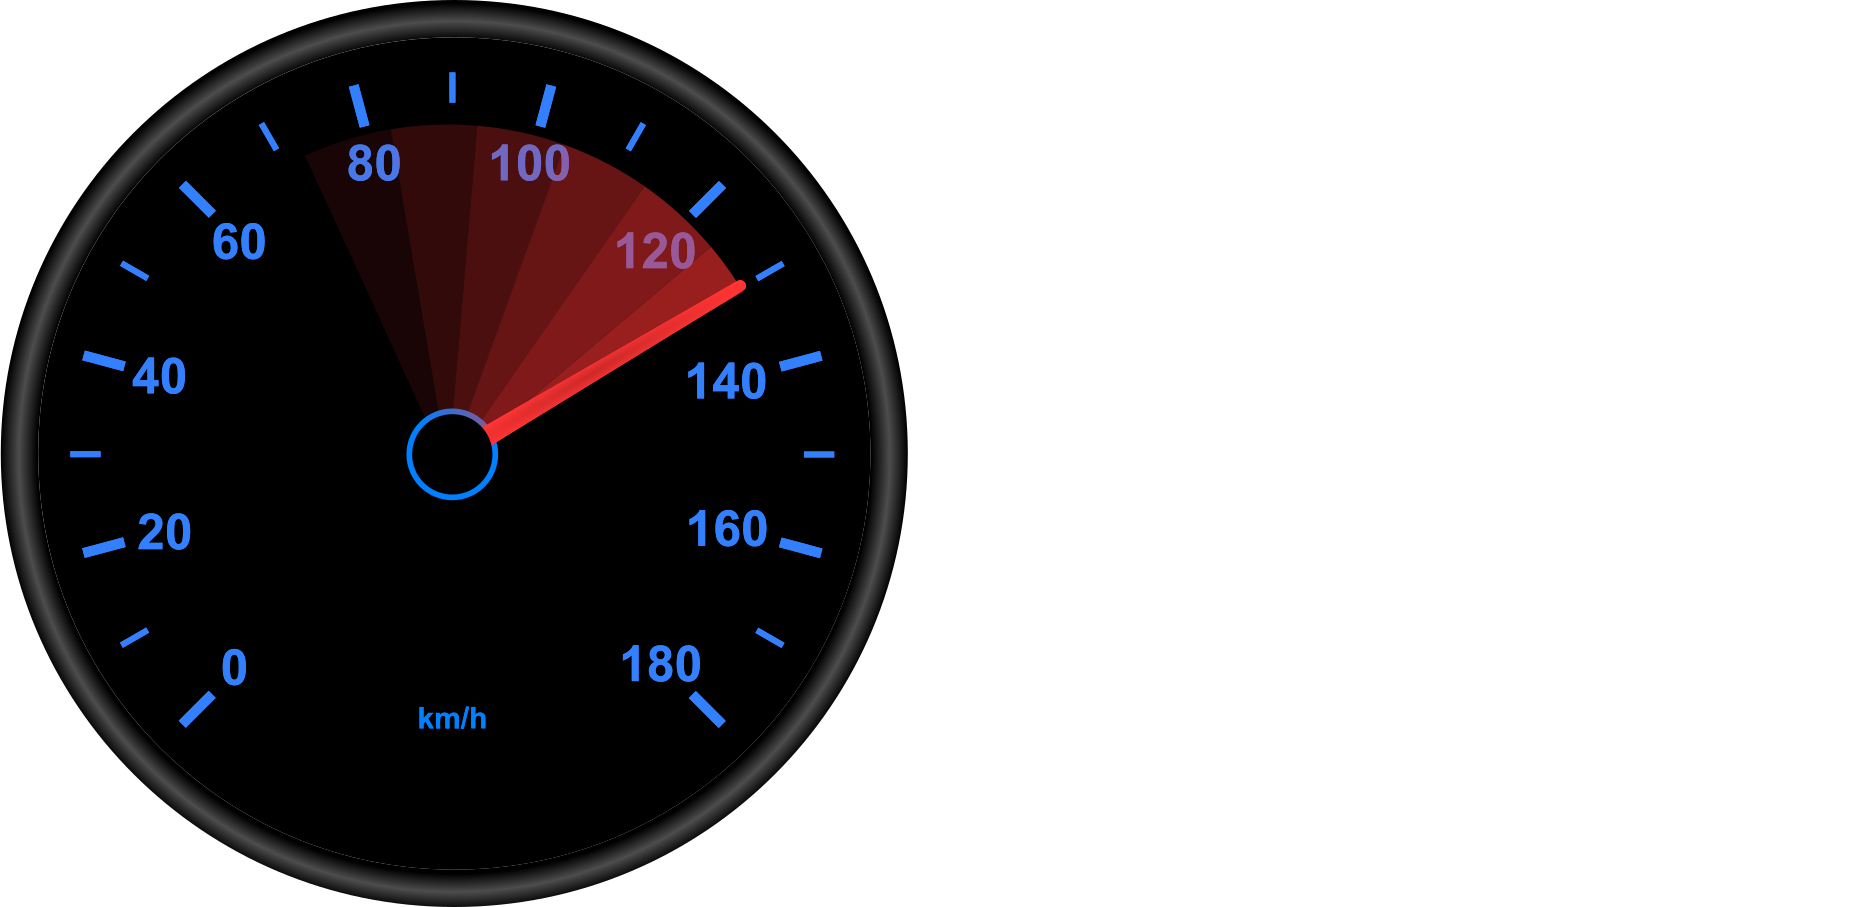
\includegraphics[width=\textwidth]{img/kmh_speedometer}
    \end{center}
    \end{column}
    \begin{column}{.48\textwidth}
      \begin{center}
        In software engineering, \textbf{profiling} ("program profiling", "software profiling") is a form of dynamic program analysis that \textbf{measures}, for example, the space (memory) or time complexity of a program, the usage of particular instructions, or frequency and duration of function calls. \textit{The most common use of profiling information is to aid program optimization.}
      \end{center}
      \begin{flushright}
        \small(\href{http://en.wikipedia.org/wiki/Profiling_(computer_programming)}{wikipedia})
      \end{flushright}

    \end{column}
  \end{columns}
\end{frame}

\subsection{\texttt{time} et al}
\begin{frame}[fragile]
\frametitle{\insertsectionhead{}: \insertsubsectionhead{}}
\vfill
\begin{block}{time}
  \begin{columns}[t]
    \begin{column}{.48\textwidth}
  \begin{pyglist}[language=bash,style=emacs]
  $ time sleep 10 #bash built-in
  
  real    0m10.001s
  user    0m0.000s
  sys     0m0.000s
\end{pyglist}  
    \end{column}
    \begin{column}{.48\textwidth}
 \begin{pyglist}[language=bash,style=emacs]
  $ `which time` -p sleep 10 \
  #unix app

  real 10.00
  user 0.00
  sys 0.00
\end{pyglist}  
    \end{column}
  \end{columns}
\end{block}
\vfill
\begin{itemize}
\item simple and effective
\item use the ``user'' time (or the wallclock time) as central measurement unit
\item CPU time is an accumulated time (does not account for waits/sleeps)
\item does apply for library based timers (\texttt{boost::cpu\_time}, \texttt{std::chrono}, \dots)
\end{itemize}
\vfill
\end{frame}

\subsection{\texttt{perf}}
\begin{frame}
\frametitle{\insertsectionhead{}: \insertsubsectionhead{}}

\end{frame}

\subsection{\texttt{valgrind}}
\begin{frame}
\frametitle{\insertsectionhead{}: \insertsubsectionhead{}}
  \begin{columns}[t]
    \begin{column}{.58\textwidth}
      \begin{itemize}
      \item originally memory profiling/debugging tool
      \item now: tool suite and framework for dynamic program analysis
      \item open-source tool under GPL
      \item runs ``instrumented'' application inside a VM
      \item apps take $2-10\times$ longer inside \texttt{valgrind}
      \end{itemize}
    \end{column}
    \begin{column}{.4\textwidth}
      \begin{center}
      \includegraphics[width=\textwidth]{img/Valgrind_logo}
    \end{center}
    
    \end{column}
  \end{columns}

\end{frame}


\part{Tour de Force}
\section{The ``Blessings'' of Design}
\subsection{Inheritance}
\begin{frame}
\frametitle{\insertsectionhead{}: \insertsubsectionhead{}}
\end{frame}

\subsection{Over-Objectivism}
\begin{frame}
\frametitle{\insertsectionhead{}: \insertsubsectionhead{}}
\end{frame}

\subsection{Take-Home}
\begin{frame}
\frametitle{\insertsectionhead{}: \insertsubsectionhead{}}
\end{frame}

\section{The Free Lunch}

\section{Vectorisation}


\part{Exercises}
\section{Tasks}
\section{Results}

\section{Literature}
\begin{frame}[c]
\frametitle{\insertsection{}}
\nocite{*}
\tiny%footnotesize
\bibliographystyle{ieeetr}
\bibliography{slides}
\end{frame}

\end{document}




